\subsection{Balance general}

Según \textcite{balance_2022} "\textit{El balance general, junto con los estados de ganancias y pérdidas, cambios en el patrimonio neto y flujos de efectivo, conforman los estados financieros básicos, cuyo propósito general es suministrar información acerca de la situación y desempeño financiero, así como de los flujos de efectivo, que sea útil a una amplia gama de usuarios al tomar sus decisiones económicas.} "

La responsabilidad de la preparación y presentación de los estados financieros recae en la administración de la empresa.

En esta oportunidad, trataremos sobre el Balance General, el cual brinda información sobre la situación financiera de una empresa al final de un periodo contable.

La información presentada en un balance general, se clasifica de manera que los usuarios obtengan información respecto a la liquidez, fecha de vencimiento de los pasivos, la cantidad de activos asignados a inmuebles, maquinarias y equipo, y la porción de activos financiados por los acreedores y por los propietarios.

La información sobre la liquidez de los activos se consigue distinguiendo entre activo corriente y no corriente. Los activos corrientes, se componen de efectivo y los recursos que se espera se conviertan en efectivo al ser vendidos o consumidos dentro de un año o en el ciclo normal de operaciones, el que sea más largo. El ciclo normal de operaciones es el periodo de tiempo, entre la compra de inventarios, el procesamiento de los inventarios para poder venderlos, la venta de los bienes y el cobro derivado de esas ventas.

La situación financiera, se representa por una serie de recursos para ser usados por la empresa, denominados activos, y las demandas sobre esos recursos representada por los pasivos y patrimonio neto.

\centerline{Patrimonio = Activos - Pasivos}

En la tabla \ref{balance} se detallan los activos, pasivos y el patrimonio de cada año tomando de inicio el año 0 con una inversión inicial de forma que inicie los procesos del negocio. En consideración con la proyección de ventas de inicia con el año contable 1 hasta el año 5.

El balance debe ser presentado para la aprobación de la Asamblea General de Accionistas por el Representante Legal con los demás documentos a que se refiere el Artículo 446 del Código de Comercio. Dentro del término establecido en la ley, El Representante Legal remitirá a la Superintendencia, si es el caso, una copia del balance y de los anexos que lo expliquen y justifiquen, junto con el Acta en que hubieren sido discutidos y aprobados.


\vspace{4mm}
\begin{minipage}{0.9\textwidth}
\centering
\captionof{table}[{Balance General }]{ Balance General }
\label{balance}
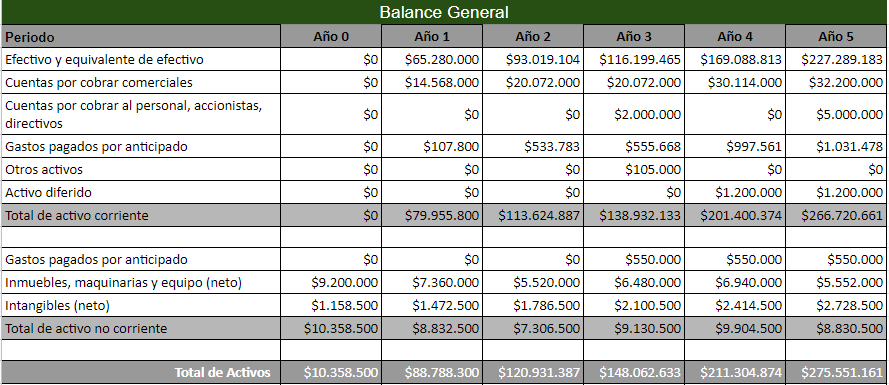
\includegraphics[width=1.1\textwidth]{Images/balance1.png}
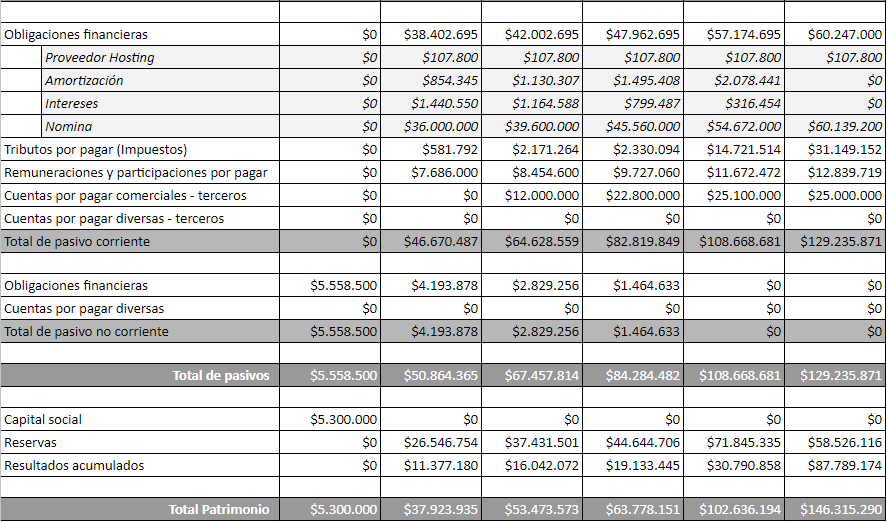
\includegraphics[width=1.1\textwidth]{Images/balance2.png}
\fnote{Nota. \textup{Fuente : Autores}}
\end{minipage}
\newpage
